\documentclass[tikz,border=8pt]{standalone}
% Shared look for every TikZ diagram. Load with \input{../../tools/tikz-style.tex}
\usepackage[T1]{fontenc}
\usepackage{lmodern}
\renewcommand{\sfdefault}{lmr}  % diagrams use the same serif as the text
\usetikzlibrary{arrows.meta, positioning, shapes.geometric, calc, fit, backgrounds}
\definecolor{cblue}{HTML}{4C78A8}
\definecolor{corange}{HTML}{F58518}
\definecolor{cgreen}{HTML}{54A24B}
\definecolor{cred}{HTML}{E45756}
\definecolor{cpurple}{HTML}{B279A2}
\definecolor{cgrey}{HTML}{6B6B6B}
\tikzset{
  every picture/.style={font=\sffamily, line width=1.2pt},
  box/.style={draw=#1, fill=#1!12, rounded corners=4pt, align=center, inner sep=7pt, minimum height=1.1cm},
  box/.default=cgrey,
  arrow/.style={-{Stealth[length=3mm]}, draw=cgrey, line width=1.4pt},
  title/.style={font=\sffamily\bfseries\Large},
  note/.style={font=\sffamily\small, text=cgrey, align=center},
}
\AtBeginDocument{\hyphenpenalty=10000 \exhyphenpenalty=10000}

\begin{document}
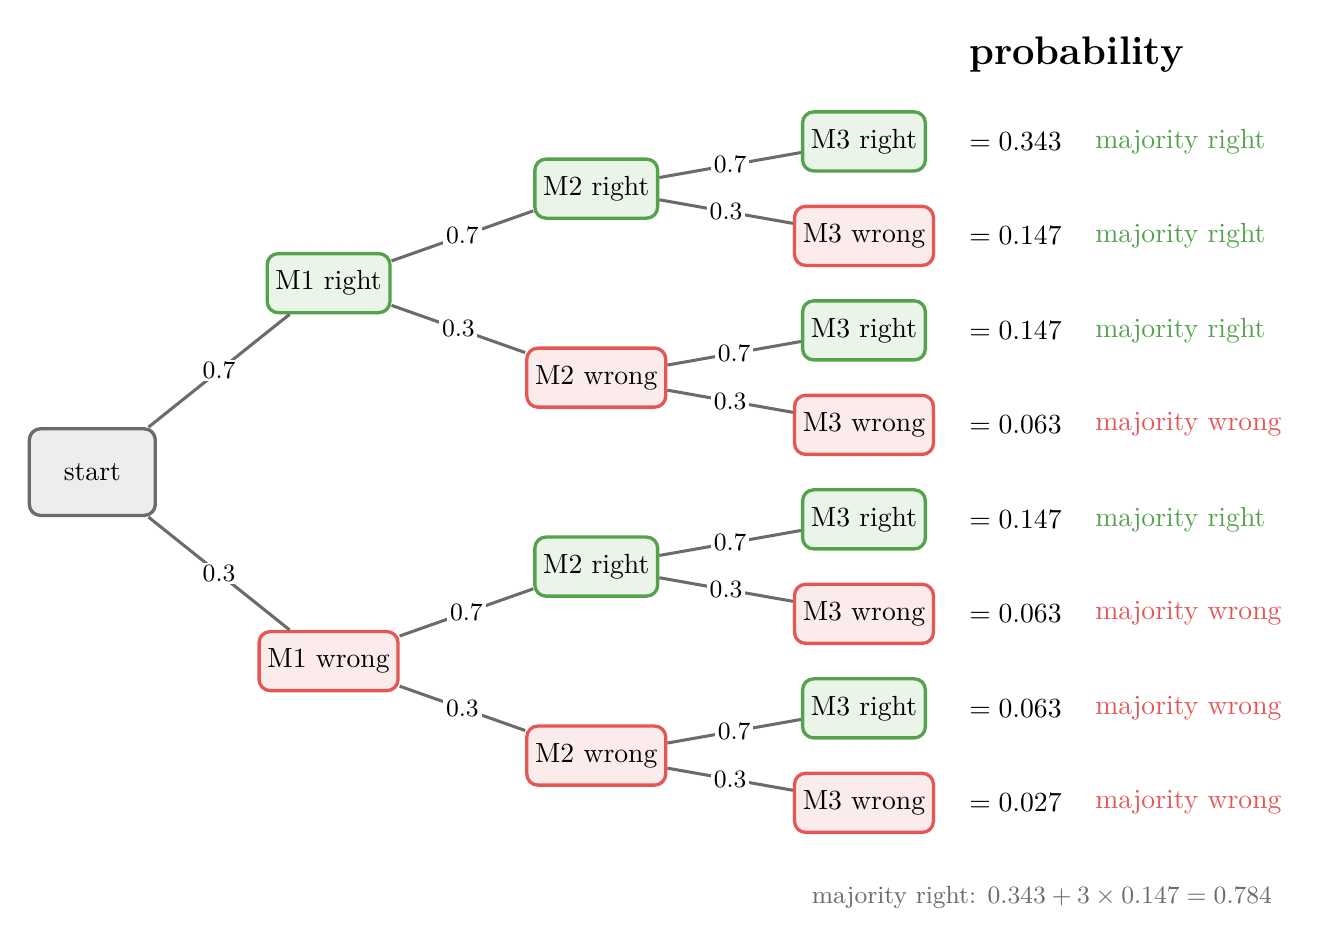
\begin{tikzpicture}[
  r/.style={box=cgreen, minimum width=1.3cm, minimum height=0.75cm, inner sep=3pt},
  w/.style={box=cred, minimum width=1.3cm, minimum height=0.75cm, inner sep=3pt},
  lab/.style={font=\sffamily\small, fill=white, inner sep=1pt},
  edge/.style={draw=cgrey, line width=1.1pt}]
  \node[box=cgrey, minimum width=1.6cm] (s) at (0,0) {start};
  % M1
  \node[r] (a) at (3,2.4) {M1 right};
  \node[w] (b) at (3,-2.4) {M1 wrong};
  \draw[edge] (s) -- node[lab] {0.7} (a); \draw[edge] (s) -- node[lab] {0.3} (b);
  % M2
  \node[r] (aa) at (6.4,3.6) {M2 right}; \node[w] (ab) at (6.4,1.2) {M2 wrong};
  \node[r] (ba) at (6.4,-1.2) {M2 right}; \node[w] (bb) at (6.4,-3.6) {M2 wrong};
  \draw[edge] (a) -- node[lab] {0.7} (aa); \draw[edge] (a) -- node[lab] {0.3} (ab);
  \draw[edge] (b) -- node[lab] {0.7} (ba); \draw[edge] (b) -- node[lab] {0.3} (bb);
  % M3 leaves: name, y, right?, product, majority right?
  \foreach \p/\y/\t/\v/\m/\maj in {aa/4.2/r/0.343/RRR/1, aa/3.0/w/0.147/RRW/1, ab/1.8/r/0.147/RWR/1, ab/0.6/w/0.063/RWW/0,
                                   ba/-0.6/r/0.147/WRR/1, ba/-1.8/w/0.063/WRW/0, bb/-3.0/r/0.063/WWR/0, bb/-4.2/w/0.027/WWW/0} {
    \ifnum\maj=1 \def\c{cgreen}\def\res{majority right}\else \def\c{cred}\def\res{majority wrong}\fi
    \node[\t] (\m) at (9.8,\y) {M3 \if\t r{}right\else{}wrong\fi};
    \draw[edge] (\p) -- node[lab] {\if\t r 0.7\else 0.3\fi} (\m);
    \node[anchor=west, font=\sffamily] at (11.0,\y) {$= \v$};
    \node[anchor=west, font=\sffamily, text=\c] at (12.6,\y) {\res};
  }
  \node[title, anchor=west] at (11.0,5.3) {probability};
  \node[note, anchor=west, align=left] at (9.0,-5.4) {majority right: $0.343 + 3 \times 0.147 = 0.784$};
\end{tikzpicture}
\end{document}
